\documentclass{scrreprt}
\usepackage{listings}
\usepackage{underscore}
\usepackage{graphicx}
\usepackage[bookmarks=true]{hyperref}
\usepackage[utf8]{inputenc}
\usepackage[french]{babel}
\renewcommand{\contentsname}{Table des matières}
\def\myversion{1.0}
\def\projectname{Le Labernois}
\hypersetup{
    bookmarks=false,    % show bookmarks bar?
    pdftitle={Cahier de charges - \projectname},    % title
    pdfauthor={Simon Landry},                       % author
    pdfsubject={Cahier de charges du site circuit voyages},  % subject of the document
    pdfkeywords={},        % list of keywords
    colorlinks=true,       % false: boxed links; true: colored links
    linkcolor=black,       % color of internal links
    citecolor=black,       % color of links to bibliography
    filecolor=black,       % color of file links
    urlcolor=blue,         % color of external links
    linktoc=page           % only page is linked
}

\usepackage{hyperref}
\begin{document}
\pagenumbering{gobble}
\begin{flushright}
    \rule{16cm}{5pt}\vskip1cm
    \begin{bfseries}
        \Huge{CAHIER DE \\ CHARGES}\\
        \vspace{1.5cm}
        pour\\
        \vspace{1.5cm}
        \projectname\\
        \vspace{1.5cm}
        \LARGE{Version \myversion}\\
        \vspace{1.5cm}
        Préparé par :\\
        Nicholas Massé\\
        Philippe Bourassa\\
        David Godin\\
        Simon Landry\\
        et Keven Aubin\\
        \vspace{1cm}
        Pour MBGLA productions\\
        \vspace{.5cm}
        8 novembre 2019\\
    \end{bfseries}
\end{flushright}
\newpage
\pagenumbering{roman}
\tableofcontents
\newpage
\pagenumbering{arabic}
\chapter{Présentation du projet}

\projectname{} est un projet destiné à mettre en place une application
web afin d'offrir des services similaires à ceux d'une agence de voyage.

\paragraph{}
Ciblant une clientèle un peu plus précise, l'entreprise a pour but
d'offrir des voyages hors normes en veillant à ce que toutes les
demandes et volontés du client soient comblées. Les offres de voyage
ont un air standardisé mais offrent un tel éventail d'options qu'elles
font plutôt partie d'une démarche «sur mesure».

\paragraph{}
Le principe de la compagnie est de développer et d'organiser des
voyages selon des thématiques spécifiques, appelées des «circuits». Les
circuits sont destinés à une clientèle internationale et se veulent
accessibles de n'importe où. Le client ayant sélectionné sa thématique
de préférence, il pourra construire son voyage en choisissant son
propre point de départ et point d'arrivée à l'intérieur du circuit
proposé.

\chapter{Objectifs et environnements}
\section{Objectifs}
Se voulant être un projet d'envergure internationale, la mise en place
de l'application \projectname{} doit passer par certaines étapes.

\paragraph{}
Tout d'abord, \projectname{} a l'intention de se démarquer de ses
concurrents par son offre de service approfondie, et devra être adaptée
à tous les types de clientèle. Malgré tout, ses services assez onéreux
forcent la compagnie à s'adresser à une clientèle plus âgée et devra
donc axer ses services dans cette direction.

\paragraph{}
\projectname{} a la volonté de devenir un leader dans les offres de
voyages de luxe, et dans cette mesure s'attend à avoir une
infrastructure technologique appropriée.


\section{Environnements}
La mise en place de l'application web inclut trois branches
principales: les environnements «Client», «Admin» et «Personnel».

\paragraph{}
L'environnement «Client» permettra à n'importe quel internaute de
naviguer sur le site et de prendre connaissance des circuits de voyage
offerts par la compagnie. Le client aura également la possibilité de
créer son compte pour avoir accès à l'inscription sur les circuits, à
des informations personnalisées, à son propre profil ainsi qu'à son
historique de voyage.

\paragraph{}
L'environnement «Admin» permettra à l'administrateur ou son mandataire
de modifier les offres de circuit, de gérer les comptes clients ainsi
que les promotions et les rabais

\paragraph{}
L'environnement «Personnel» donnera accès à la gestion des envois de
promotions et rabais. Il permettra aussi la consultation et la gestion
des paiements par les clients.

\chapter{Ressources allouées}
\section{Financement et matériel}

\projectname{} ne possède pas de limite budgétaire et c'est dans cette
optique que la qualité de l'application web doit être inégalée. Bien
qu'une limite temporelle et technologique existe, l'entreprise a
confiance en l'équipe de développement en ce qui a trait à la gestion
des ressources matérielles.

\section{Équipe de développement}

La compagnie fait appel à une équipe de jeunes développeurs composée de
finissants du niveau collégial québécois. Leurs origines
professionnelles et personnelles sont diversifiées et en font un atout
principal.

\paragraph{}
Ci-dessous se trouve un petit descriptif de chacun des membres de
l'équipe de développement.

\subsection{Keven Aubin}

Keven Aubin est un développeur web terminant sa formation au Collège de
Maisonneuve. Son expérience en développement front-end et back-end en
feront un membre polyvalent de l'équipe.

\paragraph{}
Expérimenté à la tâche de Scrum Master, Keven saura mener l'équipe dans
ce rôle lors des scrums journaliers et saura protéger l'équipe des
obstacles et distractions qui l'entourent.
Titulaire d'un diplôme de droit notarial, ce développeur utilise son
expérience de la communication pour mieux communiquer avec le client et
ainsi comprendre plus facilement les besoins et désirs du maître
d'ouvrage.

\subsection{Philippe Bourassa}

Philippe Bourassa est un développeur full-stack qui termine ses études en
informatique au Collège de Maisonneuve. Sa capacité d'apprendre par lui-même et
sa grande expérience académique aideront beaucoup son équipe à mener le projet à
terme.

\newpage

\subsection{Simon Landry}

Simon Landry est un développeur back-end terminant sa formation au Collège de
Maisonneuve. Son expertise en développement sur divers projets «Open Source»,
qui s'échelonne sur plus d'une dizaine d'années, lui permettera de conseiller
ses collègues sur les meilleures pratiques de développement et les multiple
outils qui entourent le développement. Après une année au sein des
Forces Armées Canadiennes en tant qu'officier, ce développeur saura utiliser ses
compétences en leadership pour mener le projet à termes.

\subsection{David Godin}

David Godin termine présentement ses études en informatique de gestion en tant
que programmeur analyste au Cégep de Maisonneuve tout comme le reste de ses
coéquippiers. Grâce à son experience de plus de 5 ans au sein d'une équipe
dynamique au service à la clientèle, sa capacité à communiquer et à effectuer
plusieurs tâches simultanément saura aider les membres pour la réussite de
l'équipe.

\subsection{Nicholas Massé}

Issu du domaine de la restauration et de la sommellerie, Nicholas Massé finit
présentement ses études en développement web au Collège de Maisonneuve.
Il sait donc travailler sous pression et aime relever les défis à travers les
projets qu'il entreprend. Ses connaissances en sommellerie sont aussi
étroitement liées au tourisme européen. Utilisées conjointement avec sa forte
créativité, elles feront de lui un atout majeur pour l'équipe de développement.


\chapter{Besoins}
L’application web élaborée devra permettre au propriétaire du logiciel de gérer
des circuits de voyage sur Internet ainsi qu'aux
administrateurs de la plateforme d’accéder aux informations des membres du site
et aux informations financières des commandes passées. Elle permettra également
de faire parvenir aux clients des promotions particulières, aux visiteurs de la
plateforme de consulter les différents circuits offerts à l’achat, classés par
catégorie, et de consulter les détails de ceux-ci.

\paragraph{}
Une fois enregistré et connecté à l’aide d’un compte Google ou Facebook, ou
encore à l’aide d’un nom d’utilisateur et d’un mot de passe, le visiteur
devient client enregistré et peut personnaliser son circuit. Il peut ajouter un
circuit au panier, puis commander le contenu du panier. Il peut payer l’acompte
ou toute somme restante à l’aide d’un compte PayPal. Il peut aussi modifier ou
annuler le circuit après la commande de celui-ci. Enfin, le client peut
également recevoir, s’il le désire, des promotions, des informations sur de
nouveaux circuits ou d’autres informations utiles.

\paragraph{}
Les normes graphiques du projet devront avoir été élaborées pour le projet,
incluant le choix d’une marque, d’un logo et d’une palette de couleurs.

\paragraph{}
Une API devra être développée afin de fournir les données sur les circuits à une
application mobile disponible sur la plateforme Android, elle aussi développée
dans le cadre de ce projet.


\chapter{Contraintes}
L’application devra être de type SPA (\textit{Single Page Application}) et devra être conçue avec Angular
JS, Bootstrap et JSON. Elle devra utiliser un backend PHP orienté objet ainsi
qu’une base de données MariaDB respectant les trois premières lois normales.
Toutes les données devront être validées avant d’être ajoutées à la base
de données. Les circuits en cours de création devront pouvoir être sauvegardés
afin de pouvoir être complétés plus tard. L’application web devra être hébergée
et accessible aux clients. Elle devra être disponible en français, en anglais et
en espagnol.

\chapter{Élaboration des normes graphiques}

\section{Élaboration de la marque}
Afin de bien représenter la marque auprès des clients, nous cherchions une
marque répondant à 3 critères. Elle devait être originale, simple et
disponible. Nous avons également cherché à développer une marque qui ne
mentionnait pas le voyage, afin de diversifier les produits attachés à celle-ci
au courant des prochaines années, si le client le désire.
C’est ainsi que la marque \textsc{Le labernois} a été développée. Le
labernois tire son nom d’une nouvelle race de chiens développée en 1996 au
Québec par la fondation MIRA. Créé d’un croisement entre un bouvier bernois et
d’un retriever du Labrador, ce chien a spécialement été développé afin d’offrir
aux personnes handicapées une assistance essentielle.
Le chien représente un ami, un partenaire. On lui accorde sa confiance et on
lui reconnait une grande loyauté. En choisissant une race créée au Québec, on
associe la marque à la province, sans pour autant nuire à l’exportation de la
marque.

\paragraph{}
Aucune marque n'utilise cette race de chien dans ses activités. Les noms de
domaine \texttt{labernois} et \texttt{lelabernois} ne sont pas utilisés, qu’ils
soient suivis de \texttt{.ca} ou de \texttt{.com}. Le nom est simple à retenir
et est traduisible au besoin en anglais par \textmd{The Labernese}. Les
différents noms de domaine anglophones sont tous disponibles, sauf
\texttt{labernese.com} qui est enregistré mais n’est pas utilisé.

\newpage

\section{Élaboration du logo}
Afin de bien représenter la marque, le chien devait être en mis en valeur dans
l’élaboration du logo. Il devait paraître confiant, majestueux et regarder vers
l’avenir.

\paragraph{}
Nous avons également opté pour la présence du triangle, dont les lignes droites
et précises témoignent du professionnalisme et de l’efficacité de
l’organisation. La pointe de celui-ci devra être vers la droite, afin de
témoigner d’un sentiment d’avancement, d’avenir.
Les couleurs devront être celles du chien, mais devront également s’adapter aux
couleurs choisies dans la palette de couleurs. En changeant la couleur d’un
élément de l’arrière-plan du logo tout en conservant la forme ce celui-ci, le
logo pourra s’adapter aux différents besoins visuels tout en étant facilement
identifiable.\\
\begin{center}
  
\includegraphics[width=0.5\textwidth]{images/logo.png}
\end{center}
\section{Élaboration de la palette de couleurs}
Afin de respecter les demandes du client, nous avons opté pour une palette de
couleurs rappelant les voyages. Nous avons donc opté pour des couleurs
rappelant le sable et l’eau, afin de remémorer aux clients les belles plages du
monde. Les bleus \hbox{\pdfliteral{0.36 0.74 0.90 rg}\vrule height0.2cm
width0.2cm depth0cm\pdfliteral{0 g}} serviront à attirer l’attention de
l’utilisateur de la plateforme web, alors que le crème
\hbox{\pdfliteral{0.89 0.80 0.545 rg}\vrule height0.2cm width0.2cm
depth0cm\pdfliteral{0 g}} servira de fond à nos différents éléments
graphiques. \\
\begin{center}
  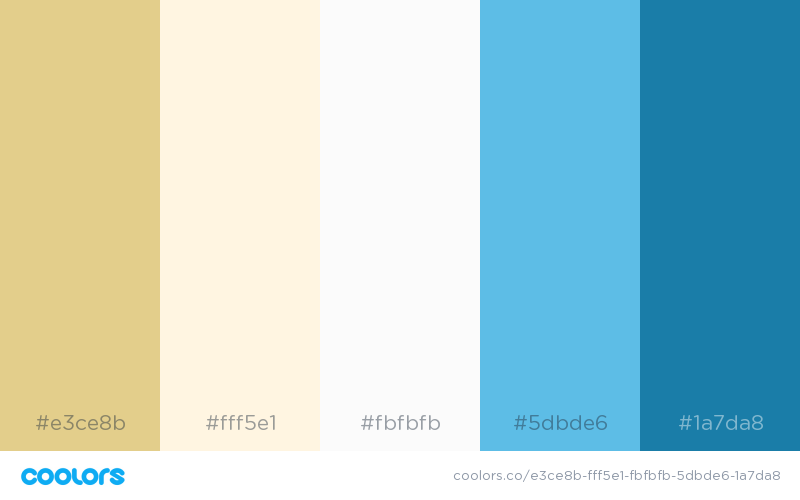
\includegraphics[width=0.5\textwidth]{images/palettev2.png}
\end{center}
\end{document}
